\chapter{Organisasi Fungsional Sel Eukariot}\label{ch:b1:eukaryotic-cell}

Sebuah \omterm{def:b1:cell-unit-of-life:cell}{sel} pankreas membuat, setiap hari, kira-kira sebanyak massanya
sendiri berupa enzim pencernaan lalu mencurahkannya ke dalam sebuah
saluran. Enzim itu adalah protein yang akan mencerna \omterm{def:b1:cell-unit-of-life:cell}{sel} yang
membuatnya; karena itu \omterm{def:b1:cell-unit-of-life:cell}{sel} itu membangunnya di dalam selembar membran
yang tertutup, mengangkutnya lewat ruang kedua tempat enzim itu dipilah
dan dipekatkan, menimbunnya dalam butiran, dan melepasnya hanya pada
isyarat sebuah santapan. Tiap langkahnya berlangsung dalam ruang
berbatas membran yang berbeda, dan lalu lintas antarruang itu diangkut
vesikel. Bab ini memerikan ruang-ruang \omterm{def:b1:cell-unit-of-life:prokeuk}{sel eukariot}, \omterm{def:b1:eukaryotic-cell:endomembrane}{sistem endomembran}
tempat protein mengalir, \omterm{def:b1:eukaryotic-cell:organelle}{organel} yang mengubah energi, rangka yang
menjaga bentuk \omterm{def:b1:cell-unit-of-life:cell}{sel} dan menggerakkan bagiannya, serta ciri yang
membedakan \omterm{def:b1:cell-unit-of-life:cell}{sel} tumbuhan dari \omterm{def:b1:cell-unit-of-life:cell}{sel} hewan.

\section{Ruang-ruang sel}

\begin{definition}[Organel, sitosol]\label{def:b1:eukaryotic-cell:organelle}
Yang disebut \emph{organel}\index{organel} adalah sebuah struktur di
dalam \omterm{def:b1:cell-unit-of-life:cell}{sel} dengan susunan dan fungsi yang tertentu; organel berbatas
membran adalah ruang yang bagian dalamnya berbeda susunannya dari
\emph{sitosol}\index{sitosol}, yaitu larutan berair \omterm{def:b1:cell-unit-of-life:cell}{sitoplasma} di
luarnya. Ruang berbatas membran: \omterm{def:b1:cell-unit-of-life:prokeuk}{inti}, \omterm{def:b1:eukaryotic-cell:endomembrane}{retikulum endoplasma}, \omterm{def:b1:eukaryotic-cell:endomembrane}{badan
Golgi}, \omterm{def:b1:eukaryotic-cell:endomembrane}{lisosom}, \omterm{def:b1:eukaryotic-cell:peroxisome}{peroksisom}, \omterm{def:b1:eukaryotic-cell:mitochondrion}{mitokondria}, dan pada tumbuhan \omterm{def:b1:eukaryotic-cell:plastid}{plastida}
serta \omterm{def:b1:eukaryotic-cell:plantcell}{vakuola}. Organel tanpa membran: ribosom, \omterm{def:b1:eukaryotic-cell:cytoskeleton}{sentrosom}, \omterm{def:b1:eukaryotic-cell:cytoskeleton}{rangka sel}.
\end{definition}

\begin{omfigure}
\begin{tikzpicture}
  \node[anchor=south west, inner sep=0] (img) at (0,0)
    {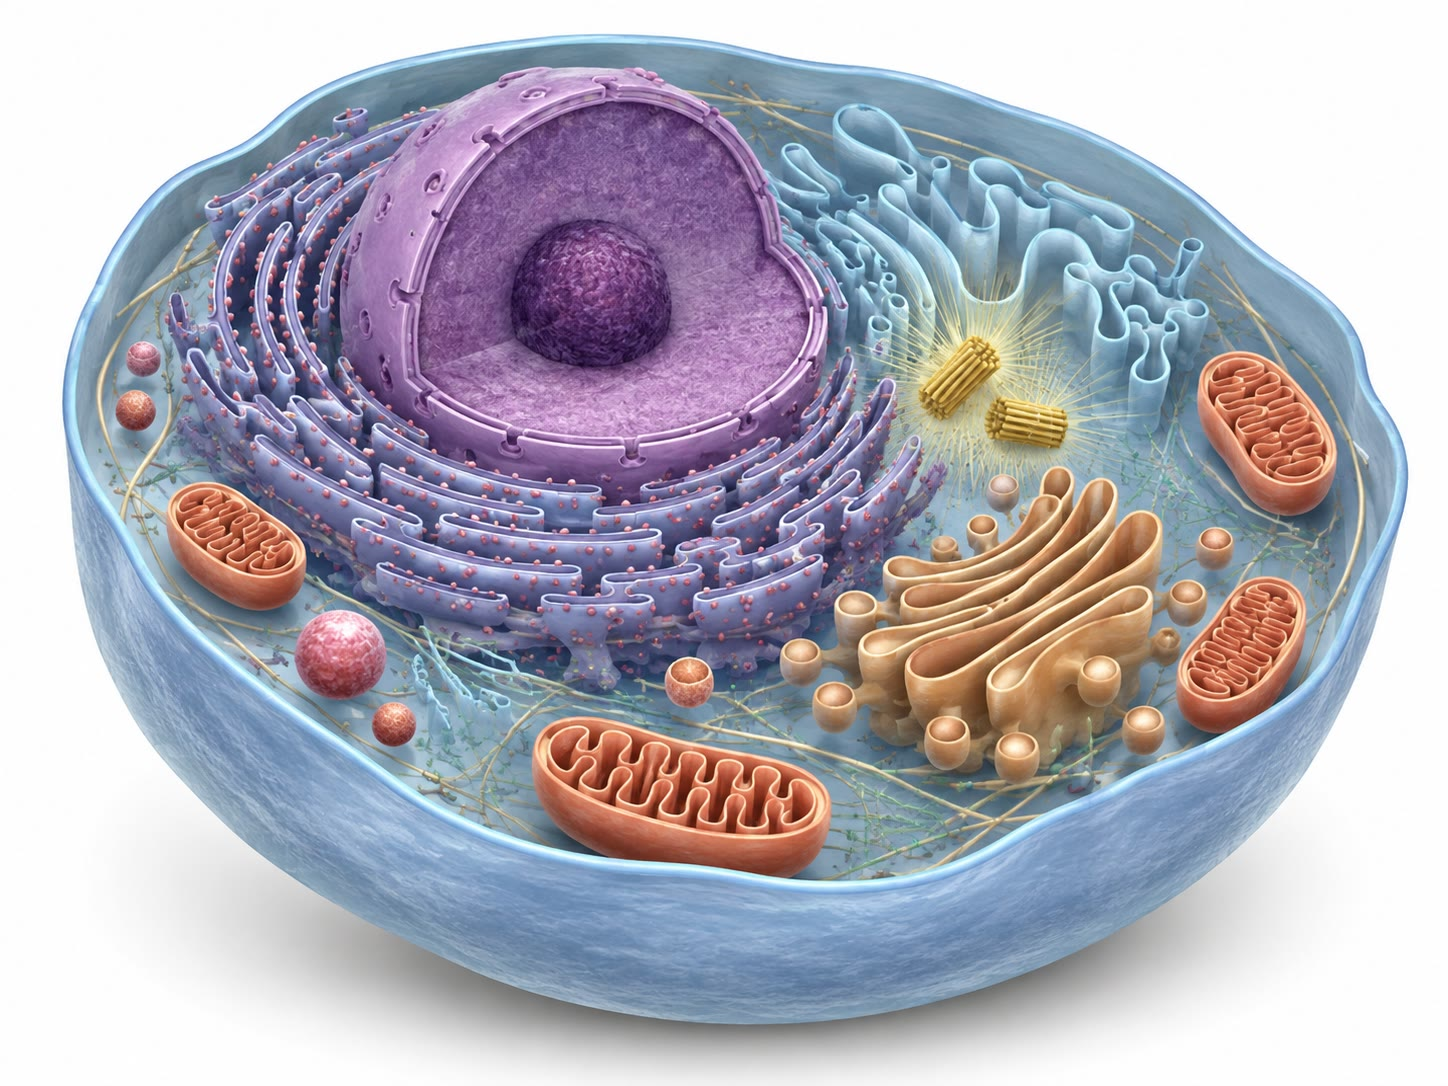
\includegraphics[width=0.6\linewidth]{images/book3/ai/fig-animal-cell-cutaway.jpg}};
  \begin{scope}[x={(img.south east)}, y={(img.north west)},
      every node/.style={font=\small}]
    \draw[omDef, thick] (0.42,0.72) -- (0.42,1.08) node[above] {inti, anak inti, liang};
    \draw[omDef, thick] (0.30,0.52) -- (-0.03,0.44) node[left, align=right] {retikulum endoplasma\\ kasar};
    \draw[omDef, thick] (0.23,0.42) -- (-0.03,0.22) node[left] {lisosom};
    \draw[omDef, thick] (0.07,0.62) -- (-0.03,0.76) node[left] {membran plasma};
    \draw[omDef, thick] (0.75,0.80) -- (1.03,0.88) node[right] {RE halus};
    \draw[omDef, thick] (0.69,0.63) -- (1.03,0.62) node[right] {sentrosom};
    \draw[omDef, thick] (0.87,0.42) -- (1.03,0.36) node[right] {mitokondria};
    \draw[omDef, thick] (0.70,0.40) -- (0.80,-0.08) node[below] {badan Golgi dan vesikelnya};
    \draw[omDef, thick] (0.47,0.25) -- (0.35,-0.08) node[below] {mitokondria};
  \end{scope}
\end{tikzpicture}

{\small Sebuah \omterm{def:b1:cell-unit-of-life:cell}{sel} hewan umum yang dibelah. \omterm{def:b1:cell-unit-of-life:prokeuk}{Intinya} di pusat; di
sekelilingnya \omterm{def:b1:eukaryotic-cell:endomembrane}{retikulum endoplasma kasar} yang bersinambung dengan
\omterm{def:b1:eukaryotic-cell:nucleus}{selubung inti}, lalu retikulum halus, tumpukan Golgi beserta vesikelnya,
\omterm{def:b1:eukaryotic-cell:mitochondrion}{mitokondria}, \omterm{def:b1:eukaryotic-cell:endomembrane}{lisosom}, dan \omterm{def:b1:eukaryotic-cell:cytoskeleton}{sentrosom} tempat \omterm{def:b1:eukaryotic-cell:cytoskeleton}{mikrotubulnya} memancar.}
\end{omfigure}

\begin{definition}[Inti sel]\label{def:b1:eukaryotic-cell:nucleus}
\emph{Inti}\index{inti sel} memegang kromosom sebagai
\emph{kromatin}\index{kromatin}, yaitu DNA yang tergulung pada protein
histon (\cref{ch:b1:genomes}). Ia dibatasi \emph{selubung
inti}\index{selubung inti}, yaitu dua membran yang bagian luarnya
bersinambung dengan \omterm{def:b1:eukaryotic-cell:endomembrane}{retikulum endoplasma}, tertembus \emph{liang
inti}\index{liang inti} tempat RNA dan protein melintas ke dua arah di
bawah kendali. \emph{Anak inti}\index{anak inti} adalah kawasan tempat
RNA ribosom dibuat dan ribosom dirakit. \omterm{def:b1:cell-unit-of-life:prokeuk}{Inti} memisahkan transkripsi (di
dalam) dari translasi (di luar), sebuah pemisahan yang tidak dimiliki
prokariot.
\end{definition}

\begin{proposition}[Ruang-ruang sebuah sel hati]\label{prop:b1:eukaryotic-cell:budget}
Dalam sebuah hepatosit bervolume \qty{5000}{\micro m^3}, \omterm{def:b1:eukaryotic-cell:organelle}{sitosolnya}
mengambil sekitar separuh volumenya, \omterm{def:b1:eukaryotic-cell:mitochondrion}{mitokondrianya} seperlima,
\omterm{def:b1:eukaryotic-cell:endomembrane}{retikulum endoplasmanya} seperenam, \omterm{def:b1:cell-unit-of-life:prokeuk}{intinya} seperenam belas, sedangkan
Golgi, \omterm{def:b1:eukaryotic-cell:endomembrane}{lisosom} dan \omterm{def:b1:eukaryotic-cell:peroxisome}{peroksisomnya} beberapa persen bersama-sama.
Membrannya bercerita lain: dari \qty{110000}{\micro m^2} membran dalam
\omterm{def:b1:cell-unit-of-life:cell}{sel} itu, separuhnya adalah \omterm{def:b1:eukaryotic-cell:endomembrane}{retikulum endoplasma}, sepertiganya membran
dalam \omterm{def:b1:eukaryotic-cell:mitochondrion}{mitokondria}, dan hanya \qty{2}{\%} membran plasma. Sebagian besar
membran sebuah \omterm{def:b1:cell-unit-of-life:cell}{sel} berada di dalamnya.
\end{proposition}

\begin{omfigure}
\begin{tikzpicture}
\begin{axis}[
  xbar, bar width=8pt,
  width=0.72\linewidth, height=6.4cm,
  axis x line=bottom, axis y line=left,
  xmin=0, xmax=45, xlabel={bagian dari seluruh membran sel (\%)},
  xlabel style={font=\small, at={(axis description cs:0.5,-0.13)}, anchor=north},
  symbolic y coords={selubung inti, membran plasma, lisosom dan peroksisom, badan Golgi, membran luar mitokondria, RE halus, membran dalam mitokondria, RE kasar},
  ytick=data, tick label style={font=\small},
  enlarge y limits=0.08, xtick={0,10,20,30,40},
  nodes near coords, nodes near coords style={font=\scriptsize, anchor=west},
]
\addplot[fill=omDef!45, draw=omDef] coordinates
  {(0.2,selubung inti) (2,membran plasma) (1.5,lisosom dan peroksisom) (7,badan Golgi) (7,membran luar mitokondria) (16,RE halus) (32,membran dalam mitokondria) (35,RE kasar)};
\end{axis}
\end{tikzpicture}

{\small Tempat membran sebuah \omterm{def:b1:cell-unit-of-life:cell}{sel} hati berada. Membran plasma,
satu-satunya yang tampak dari luar, adalah dua persen totalnya;
retikulumnya dan membran dalam \omterm{def:b1:eukaryotic-cell:mitochondrion}{mitokondrianya}, yang terlipat di dalam,
adalah empat perlimanya.}
\end{omfigure}

\section{Sistem endomembran}

\begin{definition}[Retikulum endoplasma, badan Golgi, lisosom]\label{def:b1:eukaryotic-cell:endomembrane}
Yang disebut \emph{retikulum endoplasma}\index{retikulum endoplasma}
(RE) adalah sebuah jala lembaran dan pipa membran yang melingkupi satu
ruang bersinambung, yaitu lumennya, dan bersinambung dengan \omterm{def:b1:eukaryotic-cell:nucleus}{selubung
inti}. Bagiannya yang \emph{kasar}\index{retikulum endoplasma kasar}
bertaburan ribosom yang menyuntikkan protein buatannya ke dalam lumen
atau ke dalam membrannya; bagiannya yang \emph{halus}\index{retikulum endoplasma halus}
membuat lipid, menimbun kalsium dan menawarkan racun.
\emph{Badan Golgi}\index{badan Golgi} adalah setumpuk kantong pipih
(sisterna), dengan sisi \emph{cis} penerima dekat RE dan sisi
\emph{trans} pengirim, tempat protein dari RE diubah (gulanya dipangkas
dan ditambahkan), dipilah, dan dikemas ke dalam vesikel menuju
tujuannya. \emph{Lisosom}\index{lisosom} adalah vesikel yang asam (pH
$\approx 5$) dan penuh enzim hidrolitik yang mencerna bahan yang dibawa
masuk dari luar atau \omterm{def:b1:eukaryotic-cell:organelle}{organel} yang sudah aus. Bersama vesikel yang
bergerak di antaranya dan membran plasma, semuanya membentuk \emph{sistem
endomembran}\index{sistem endomembran}: satu himpunan ruang yang
terhubung dan lumennya secara topologis adalah sisi luar \omterm{def:b1:cell-unit-of-life:cell}{sel}.
\end{definition}

\begin{proposition}[Lintasan sekresi]\label{prop:b1:eukaryotic-cell:secretory}
\index{lintasan sekresi}
Sebuah protein yang ditakdirkan untuk disekresikan, untuk membran
plasma, atau untuk sebuah \omterm{def:b1:eukaryotic-cell:endomembrane}{lisosom} disintesis oleh ribosom yang terikat
pada RE kasar, masuk ke lumen RE sambil dibuat, melipat di sana,
mengembara dalam vesikel ke sisi cis Golgi, melintasi tumpukan itu
sambil diubah, dan meninggalkan sisi trans dalam sebuah vesikel yang
teralamatkan ke tujuannya: sebuah butiran sekresi yang melebur dengan
membran plasma pada sebuah isyarat (\emph{eksositosis
teratur}\index{eksositosis}), sebuah vesikel yang melebur terus-menerus
(eksositosis \emph{konstitutif}, yang juga mengantarkan membran baru),
atau sebuah \omterm{def:b1:eukaryotic-cell:endomembrane}{lisosom}. Protein \omterm{def:b1:eukaryotic-cell:organelle}{sitosol} dan protein \omterm{def:b1:cell-unit-of-life:prokeuk}{inti} dibuat pada
ribosom bebas dan tak pernah masuk ke sistem itu. Yang menentukan adalah
sebuah \emph{urutan isyarat}\index{urutan isyarat} pada awal protein
tersebut (\cref{ch:b1:gene-expression}).
\end{proposition}
\begin{proof}[Bukti eksperimental]
Palade (tahun 1960-an) memberi makan irisan pankreas marmot dengan asam
amino radioaktif selama tiga menit (\emph{denyutnya}), lalu asam amino tak
bertanda (\emph{pengejarannya}), dan menemukan letak keradioaktifannya
lewat autoradiografi mikrograf elektron pada beberapa selang. Pada
\qty{3}{min} butir peraknya terletak di atas RE kasar; pada
\qty{20}{min} di atas Golgi; pada \qty{40}{min} di atas \omterm{def:b1:eukaryotic-cell:plantcell}{vakuola}
pemekat dan butiran baru; pada \qty{2}{h} di dalam lumen salurannya.
\omterm{def:b1:cell-unit-of-life:fractionation}{Fraksinasi sel} memberikan urutan yang sama secara kimia. Blobel (tahun
1970-an) memperlihatkan bahwa protein sekresi yang dibuat dalam tabung
uji tanpa membran dua puluh residu lebih panjang daripada bentuk yang
disekresikan dan tidak terlindung dari protease yang ditambahkan,
sedangkan bila dibuat dengan membran RE hadir protein itu terpotong dan
terlindung: residu tambahan itulah isyarat yang mengarahkan rantai yang
sedang tumbuh masuk ke RE.
\end{proof}

\begin{omfigure}
\begin{tikzpicture}
\begin{axis}[
  width=0.9\linewidth, height=6.2cm,
  axis x line=bottom, axis y line=left,
  xmin=0, xmax=130, ymin=0, ymax=105,
  xlabel={waktu sesudah denyutnya (min)}, ylabel={bagian dari tandanya (\%)},
  xlabel style={font=\small, at={(axis description cs:0.5,-0.12)}, anchor=north},
  ylabel style={font=\small},
  tick label style={font=\small}, xtick={0,20,40,60,80,100,120}, ytick={0,25,50,75,100},
  legend style={font=\small, at={(0.5,-0.24)}, anchor=north, draw=none, legend columns=2, /tikz/every even column/.append style={column sep=0.4cm}},
  clip=false,
]
\addplot[very thick, omDef, smooth] coordinates {(3,88) (7,55) (15,25) (30,8) (60,2) (120,0)};
\addlegendentry{RE kasar}
\addplot[very thick, omProp, smooth] coordinates {(3,8) (7,35) (15,55) (30,35) (60,10) (120,2)};
\addlegendentry{Golgi dan vakuola pemekat}
\addplot[very thick, omThm, smooth] coordinates {(3,0) (7,3) (15,12) (30,45) (60,70) (90,55) (120,30)};
\addlegendentry{butiran sekresi}
\addplot[very thick, omExo, smooth] coordinates {(3,0) (7,0) (15,0) (30,2) (60,12) (90,35) (120,65)};
\addlegendentry{disekresikan ke dalam salurannya}
\end{axis}
\end{tikzpicture}

{\small Denyut dan pengejaran Palade pada pankreas: tempat protein
bertanda itu berada, sebagai fungsi waktu. Protein itu berpindah dari
RE ke Golgi dalam seperempat jam, mencapai butirannya dalam satu jam,
dan meninggalkan \omterm{def:b1:cell-unit-of-life:cell}{selnya} sepanjang dua jam berikutnya.}
\end{omfigure}

\begin{omfigure}
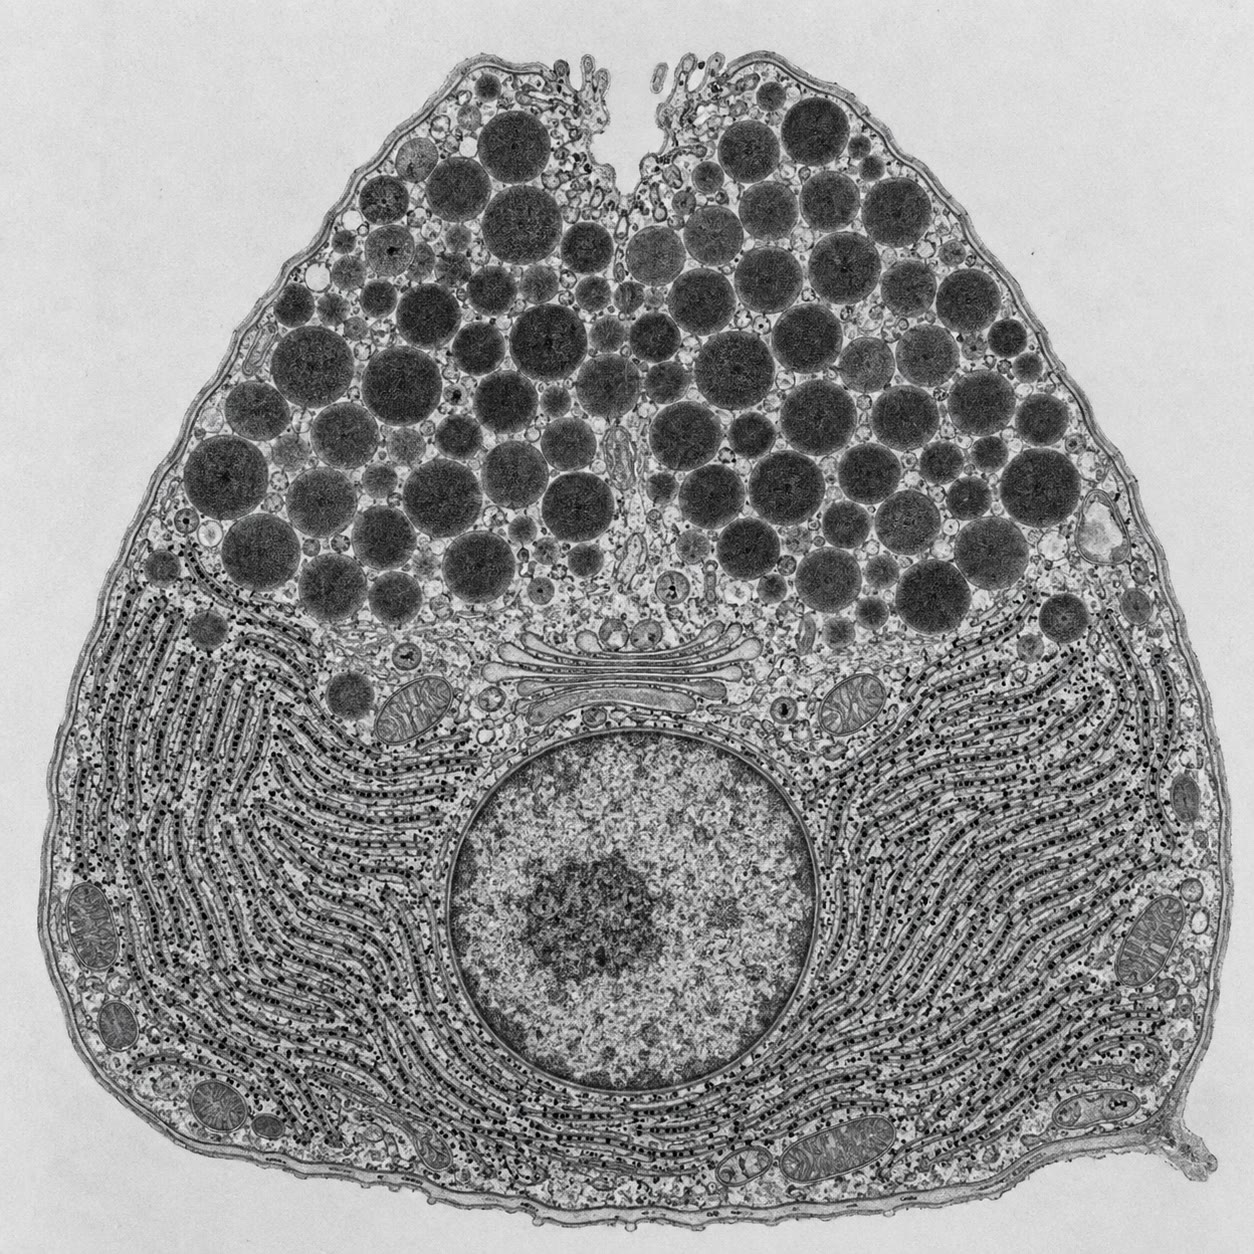
\includegraphics[width=0.44\linewidth]{images/book3/ai/b3-06-acinar-cell-tem.jpg}

{\small Sebuah \omterm{def:b1:cell-unit-of-life:cell}{sel} asinus pankreas dalam \omterm{prop:b1:cell-unit-of-life:microscopes}{mikroskop elektron} transmisi:
RE kasar yang berjejal dalam tumpukan sejajar mengelilingi \omterm{def:b1:cell-unit-of-life:prokeuk}{inti} di
pangkalnya, Golgi di atasnya, dan butiran sekresi yang padat berdesakan
ke arah puncaknya dan salurannya.}
\end{omfigure}

\begin{method}[Mengikuti sebuah molekul menembus sel]\label{met:b1:eukaryotic-cell:pulsechase}
\begin{enumerate}
  \item Tandailah satu rombongan pendek: paparkan \omterm{def:b1:cell-unit-of-life:cell}{sel} pada sebuah
        prazat radioaktif atau berpendar selama beberapa menit
        (denyutnya), lalu gantilah dengan prazat tak bertanda yang
        berlebih (pengejarannya), sehingga hanya molekul yang dibuat
        selama denyutnya yang membawa tanda itu.
  \item Ambillah cuplikan pada beberapa selang, fiksasi, lalu temukan
        letak tandanya: lewat autoradiografi sayatan, lewat mikroskopi
        fluoresensi, atau lewat fraksinasi dan pencacahan.
  \item Ruang yang tandanya memuncak lebih dahulu berada di hulu;
        urutan puncaknya adalah rutenya; selangnya adalah waktu
        singgahnya.
  \item Hambatlah satu langkah (dingin, penghambat energi, sebuah
        mutan) lalu lihatlah di mana tandanya menumpuk: ruang sebelum
        hambatan itu.
\end{enumerate}
\end{method}

\begin{definition}[Endositosis]\label{def:b1:eukaryotic-cell:endocytosis}
Yang disebut \emph{endositosis}\index{endositosis} membawa bahan masuk:
membran plasma melekuk ke dalam mengelilinginya lalu menjepit sebuah
vesikel, yang umumnya melebur dengan sebuah \omterm{def:b1:eukaryotic-cell:endomembrane}{lisosom}.
\emph{Fagositosis} menelan partikel (sebuah bakteri, sebuah \omterm{def:b1:cell-unit-of-life:cell}{sel} yang
mati); \emph{pinositosis} memasukkan tetesan cairan; \emph{endositosis
berperantara reseptor} memekatkan satu molekul tertentu (partikel
pembawa kolesterol, transferin pembawa besi) pada reseptor di dalam
lekuk bersalut sebelum memasukkannya. Eksositosis menambahkan membran
pada permukaan \omterm{def:b1:cell-unit-of-life:cell}{sel} dan endositosis menyingkirkannya; pada \omterm{def:b1:cell-unit-of-life:cell}{sel} yang
menyekresi keduanya berimbang sehingga permukaannya tetap sementara
seluruh bidang membran berputar melewatinya tiap jam.
\end{definition}

\section{Mitokondria dan plastida}

\begin{definition}[Mitokondria]\label{def:b1:eukaryotic-cell:mitochondrion}
Yang disebut \emph{mitokondria}\index{mitokondria} adalah \omterm{def:b1:eukaryotic-cell:organelle}{organel}
selebar \qtyrange{0.5}{1}{\micro m} dan sepanjang beberapa mikrometer,
yang dibatasi dua membran: membran luar yang licin dan tertembus
molekul kecil, serta membran dalam yang terlipat menjadi
\emph{krista}\index{krista} yang tak tertembus ion dan membawa rantai
respirasi serta ATP sintase (\cref{ch:b1:respiration-fermentation}). Di
dalamnya terdapat \emph{matriks}\index{matriks mitokondria}, yang
memegang enzim daur Krebs, ribosom bertipe bakteri dan beberapa salinan
DNA melingkar yang kecil. Mitokondria membelah lewat pembelahan
biner, bergerak sepanjang \omterm{def:b1:eukaryotic-cell:cytoskeleton}{rangka sel}, dan berjumlah dari beberapa ratus
sampai beberapa ribu tiap \omterm{def:b1:cell-unit-of-life:cell}{sel}.
\end{definition}

\begin{definition}[Plastida]\label{def:b1:eukaryotic-cell:plastid}
Yang disebut \emph{plastida}\index{plastida} adalah \omterm{def:b1:eukaryotic-cell:organelle}{organel} bermembran
rangkap pada \omterm{def:b1:cell-unit-of-life:cell}{sel} tumbuhan: \emph{kloroplas}\index{kloroplas}, yang di
dalamnya sistem membran ketiga, yaitu \emph{tilakoid}\index{tilakoid}
yang bertumpuk menjadi grana dan terendam dalam
\emph{stroma}\index{stroma}, menjalankan fotosintesis
(\cref{ch:b1:photosynthesis}); amiloplas, yang menimbun pati;
kromoplas, yang memegang pigmen buah dan mahkota bunga. Semuanya
diturunkan dari proplastida dan, seperti \omterm{def:b1:eukaryotic-cell:mitochondrion}{mitokondria}, memuat DNA
melingkarnya sendiri serta ribosom bertipe bakteri dan membelah lewat
pembelahan biner.
\end{definition}

\begin{omfigure}
\begin{minipage}[b]{0.48\linewidth}\centering
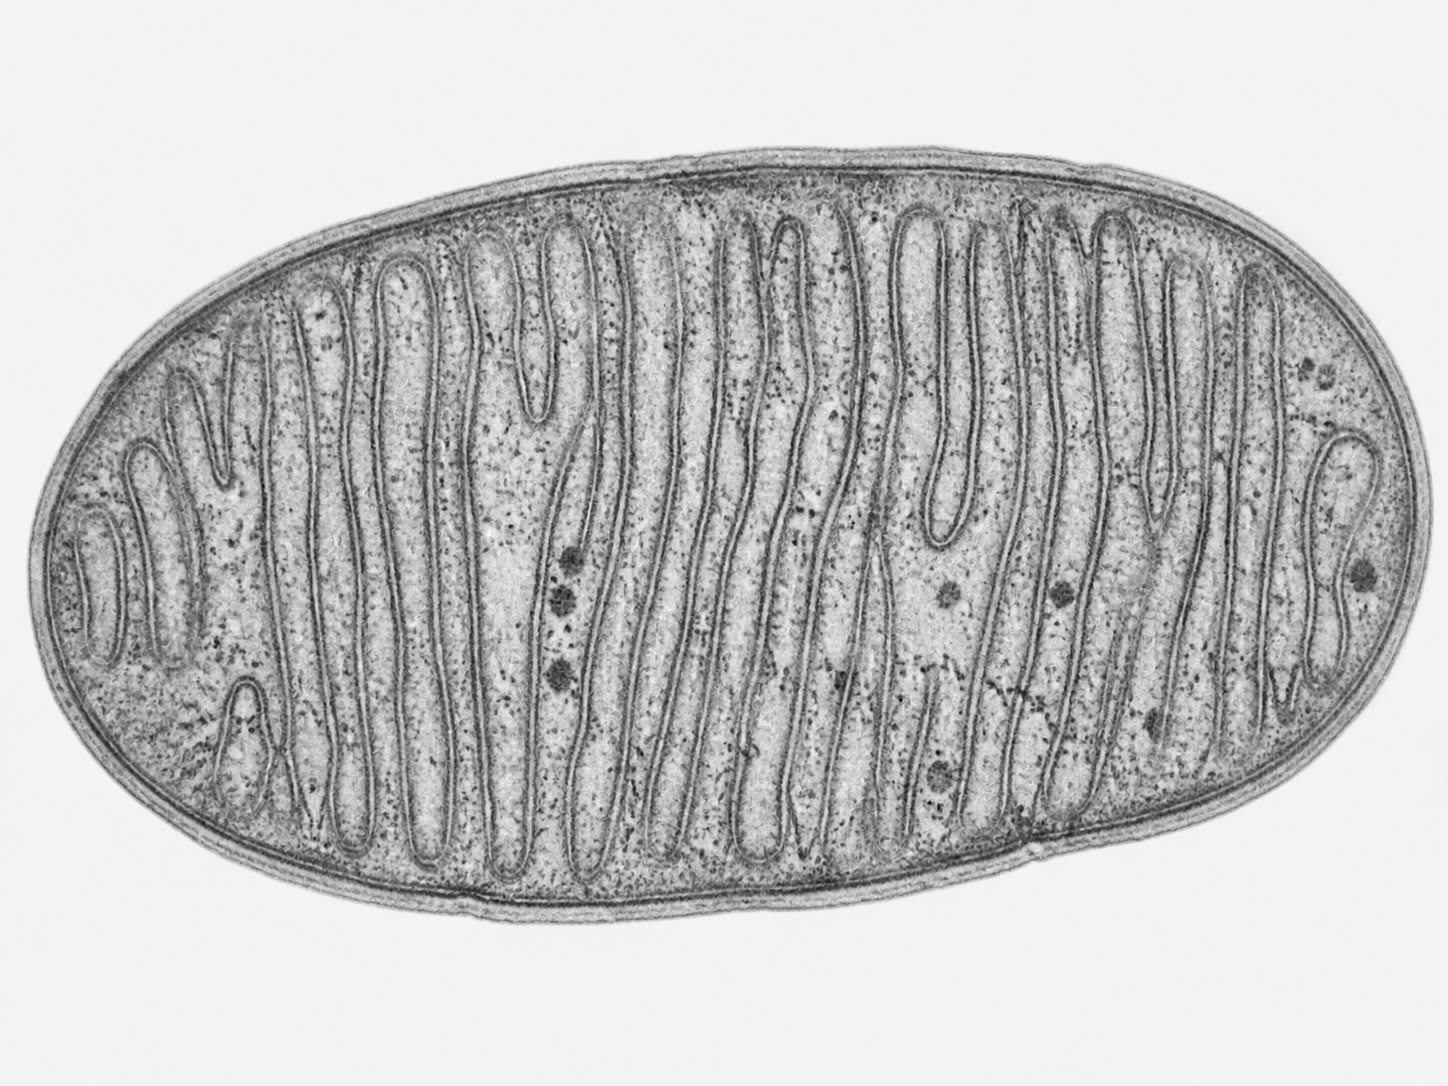
\includegraphics[width=0.96\linewidth]{images/book2/ai/g12-resp-mitochondrion-tem.jpg}
\end{minipage}\hfill
\begin{minipage}[b]{0.48\linewidth}\centering
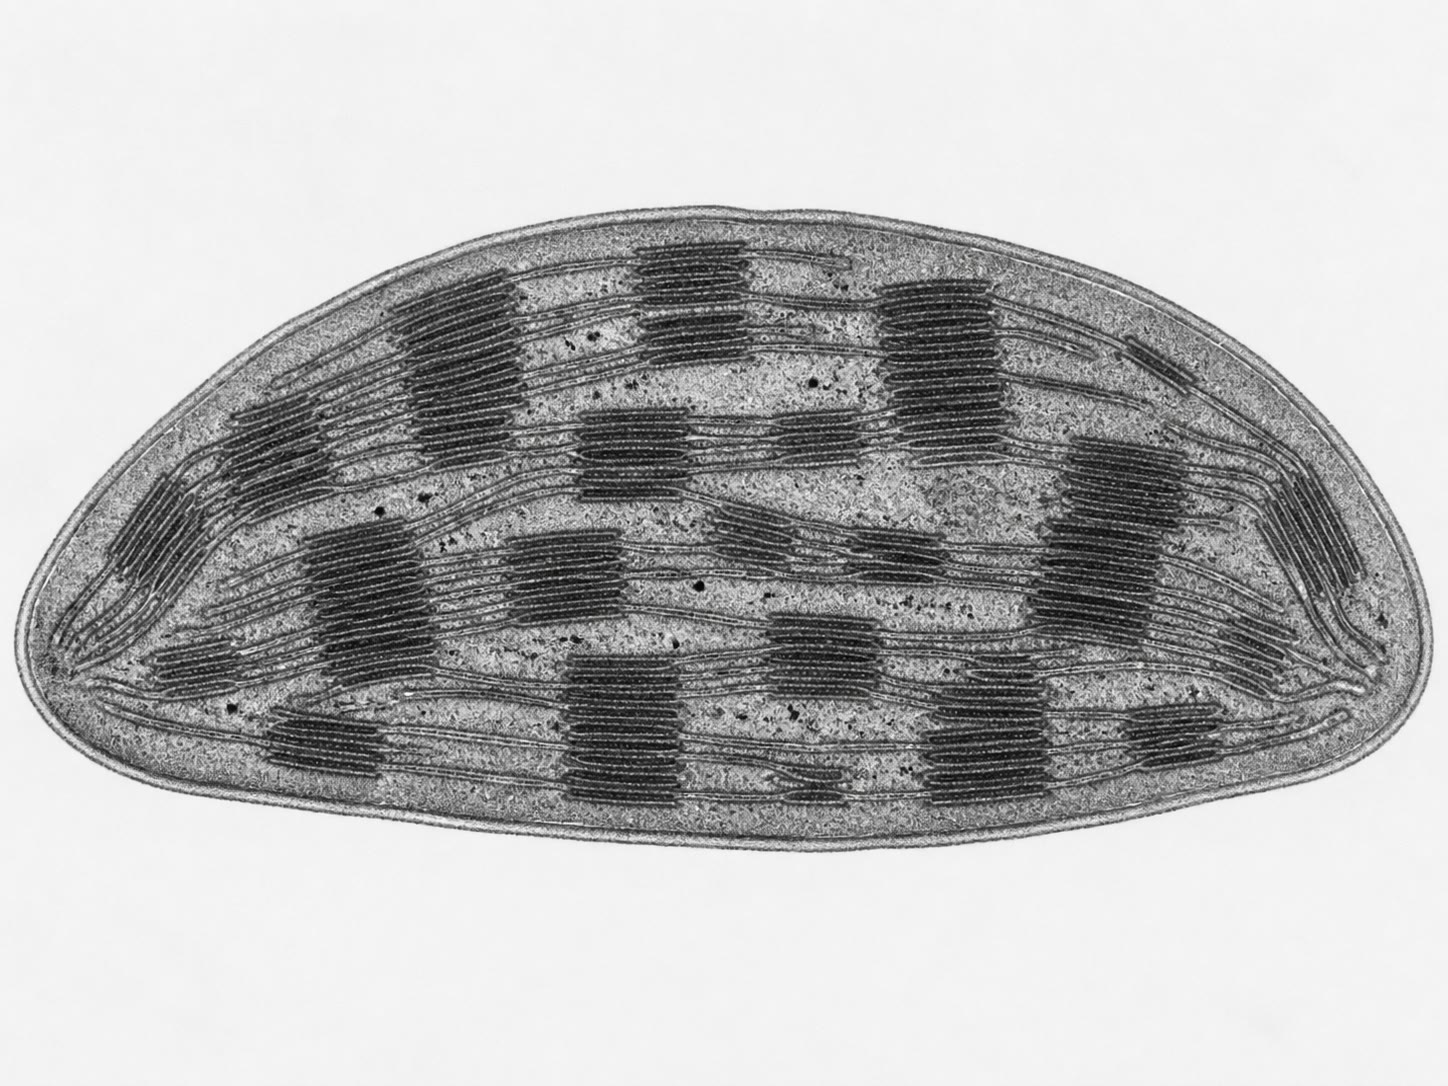
\includegraphics[width=0.96\linewidth]{images/book2/ai/g12-photo-chloroplast-tem.jpg}
\end{minipage}

{\small Sebuah \omterm{def:b1:eukaryotic-cell:mitochondrion}{mitokondria} (kiri) dan sebuah \omterm{def:b1:eukaryotic-cell:plastid}{kloroplas} (kanan) dalam
sayatan di bawah \omterm{prop:b1:cell-unit-of-life:microscopes}{mikroskop elektron}. Masing-masing bermembran selubung
dua lapis; di dalamnya, membran dalam \omterm{def:b1:eukaryotic-cell:mitochondrion}{mitokondria} yang terlipat dan
\omterm{def:b1:eukaryotic-cell:plastid}{tilakoid} \omterm{def:b1:eukaryotic-cell:plastid}{kloroplas} yang bertumpuk --- membran tempat energi diubah.}
\end{omfigure}

\begin{proposition}[Asal usul endosimbiosis]\label{prop:b1:eukaryotic-cell:endosymbiosis}
\index{endosimbiosis}
\omterm{def:b1:eukaryotic-cell:mitochondrion}{Mitokondria} dan \omterm{def:b1:eukaryotic-cell:plastid}{plastida} diturunkan dari bakteri yang hidup bebas lalu
ditelan sebuah \omterm{def:b1:cell-unit-of-life:prokeuk}{sel eukariot} leluhur dan dipertahankan sebagai simbion:
\omterm{def:b1:eukaryotic-cell:mitochondrion}{mitokondria} dari sebuah bakteri aerob, \omterm{def:b1:eukaryotic-cell:plastid}{plastida} dari sebuah sianobakteri.
\end{proposition}
\begin{proof}[Bukti eksperimental]
Kedua \omterm{def:b1:eukaryotic-cell:organelle}{organel} itu bermembran dua, yang di dalam bersusunan bakteri dan
yang di luar mirip milik inangnya; berkromosom melingkar tanpa histon;
beribosom seukuran ribosom bakteri dan peka terhadap antibiotik;
berkode genetik dengan ragam bakteri; membelah secara biner lepas dari
pembelahan \omterm{def:b1:cell-unit-of-life:cell}{selnya}; dan gennya, ketika diurutkan, mengelompok bersama
gen garis keturunan bakteri tertentu (alfaproteobakteri, sianobakteri)
alih-alih bersama gen \omterm{def:b1:eukaryotic-cell:nucleus}{inti sel} yang menaunginya. Sebagian besar gen
aslinya sejak itu telah berpindah ke \omterm{def:b1:cell-unit-of-life:prokeuk}{inti}, dan \omterm{def:b1:eukaryotic-cell:organelle}{organel} itu tidak lagi
sanggup hidup sendirian.
\end{proof}

\begin{definition}[Peroksisom]\label{def:b1:eukaryotic-cell:peroxisome}
Yang disebut \emph{peroksisom}\index{peroksisom} adalah \omterm{def:b1:eukaryotic-cell:organelle}{organel} kecil
bermembran tunggal yang memuat enzim oksidatif yang memindahkan
hidrogen dari substratnya (asam lemak, alkohol) ke oksigen, sehingga
menghasilkan hidrogen peroksida, serta katalase, yang memusnahkan
peroksida itu di tempat. Ia mengurung sebuah kimia yang berbahaya.
\end{definition}

\section{Rangka sel}

\begin{definition}[Rangka sel]\label{def:b1:eukaryotic-cell:cytoskeleton}
Yang disebut \emph{rangka sel}\index{rangka sel} adalah sebuah jala
filamen protein yang memberi \omterm{def:b1:cell-unit-of-life:cell}{sel} bentuknya, menambatkan \omterm{def:b1:eukaryotic-cell:organelle}{organelnya}, dan
menggerakkan \omterm{def:b1:eukaryotic-cell:organelle}{organel} itu serta \omterm{def:b1:cell-unit-of-life:cell}{selnya} sendiri. Ada tiga macam:
\emph{mikrofilamen}\index{mikrofilamen} dari aktin (\qty{7}{nm}, dua
untai terpilin dari subunit bulat), yang memusat di bawah membran
plasma dan bertanggung jawab atas bentuk \omterm{def:b1:cell-unit-of-life:cell}{sel}, gerak merayap, cincin
kerut pembelahan dan kerutan otot bersama miosin;
\emph{mikrotubul}\index{mikrotubul} (pipa berongga \qty{25}{nm} dari
tubulin), yang memancar dari \emph{sentrosom}\index{sentrosom}, yaitu
rel tempat protein motor (kinesin ke arah luar, dinein ke arah dalam)
membawa vesikel dan \omterm{def:b1:eukaryotic-cell:organelle}{organel}, gelendong pembelahan, serta teras silia
dan flagel; \emph{filamen antara}\index{filamen antara} (\qty{10}{nm},
serupa tali, dari keratin dan protein kerabatnya), yaitu serabut yang
tahan secara mekanis yang mengakukan \omterm{def:b1:cell-unit-of-life:cell}{sel} dan menambat pada desmosom.
Mikrofilamen dan mikrotubul merakit dan membongkar diri terus-menerus
dari lubuk subunitnya.
\end{definition}

\begin{omfigure}
\begin{tikzpicture}[font=\footnotesize, line cap=round]
  % actin: two twisted strands of beads
  \foreach \i in {0,...,15} {
    \pgfmathsetmacro{\y}{0.13*sin(\i*45)}
    \fill[omThm!70] (0.35*\i,1.6+\y) circle (0.11);
    \fill[omThm!45] (0.35*\i+0.17,1.6-\y) circle (0.11);
  }
  \node[anchor=west, align=left] at (6.0,1.6) {\textbf{mikrofilamen} (aktin), \qty{7}{nm}\\ bentuk, gerak merayap, cincin pembelahan, otot};
  % intermediate filament: rope of coiled strands
  \foreach \k in {0,1,2,3} {
    \draw[omProp, thick] plot[domain=0:5.3, samples=60] (\x, {0.55+0.09*sin(180*\x+90*\k)});
  }
  \node[anchor=west, align=left] at (6.0,0.55) {\textbf{filamen antara}, \qty{10}{nm}\\ serupa tali, kekuatan mekanis};
  % microtubule: hollow tube of protofilaments
  \draw[thick, omDef!70!black, fill=omDef!15] (0,-0.9) rectangle (5.3,-0.2);
  \foreach \i in {0,...,25} { \foreach \j in {0,1,2,3} {
    \fill[omDef!60] (0.1+0.2*\i, -0.83+0.19*\j) circle (0.075);
  } }
  \draw[thick, omDef!70!black, fill=omDef!10] (5.3,-0.55) ellipse (0.18 and 0.35);
  \draw[thick, omDef!70!black, fill=white] (5.3,-0.55) ellipse (0.10 and 0.24);
  \node[anchor=west, align=left] at (6.0,-0.55) {\textbf{mikrotubul} (tubulin), \qty{25}{nm} berongga\\ rel bagi motor, gelendong, silia};
\end{tikzpicture}

{\small Ketiga filamen \omterm{def:b1:eukaryotic-cell:cytoskeleton}{rangka sel}, digambar pada skala yang sama. Aktin
dan tubulin berpolimerisasi secara berbalikan dari subunit bulat;
\omterm{def:b1:eukaryotic-cell:cytoskeleton}{filamen antara} adalah tali yang mantap.}
\end{omfigure}

\begin{example}[Menggerakkan sebuah vesikel]\label{ex:b1:eukaryotic-cell:transport}
Sebuah vesikel sekresi yang meninggalkan Golgi dijemput kinesin, sebuah
motor yang berjalan sepanjang sebuah \omterm{def:b1:eukaryotic-cell:cytoskeleton}{mikrotubul} ke arah tepi \omterm{def:b1:cell-unit-of-life:cell}{sel} pada
sekitar \qty{1}{\micro m/s}, dengan biaya satu ATP tiap langkah
\qty{8}{nm}; dalam sebuah \omterm{def:b1:body-plans-tissues:nervous}{neuron} motor yang sama membawa vesikel
sepanjang sebuah akson yang panjangnya semeter --- sebuah perjalanan
sepuluh hari. Dekat permukaannya, vesikel itu diserahkan ke korteks
aktin dan ke miosin bagi mikrometer terakhirnya. Difusi akan membuat
sebuah vesikel \qty{100}{nm} butuh sekitar semenit untuk melintasi \omterm{def:b1:cell-unit-of-life:cell}{sel}
\qty{20}{\micro m}, dan bertahun-tahun untuk menempuh semeter: \omterm{def:b1:eukaryotic-cell:organelle}{organel}
diangkut, bukan dibiarkan mengembara.
\end{example}

\section{Sel tumbuhan dan sel hewan}

\begin{definition}[Dinding sel, vakuola, plasmodesmata]\label{def:b1:eukaryotic-cell:plantcell}
Sebuah \omterm{def:b1:cell-unit-of-life:cell}{sel} tumbuhan menambahkan tiga struktur pada rancangan bersama
itu. \emph{Dinding sel}\index{dinding sel}, di luar membran plasma,
adalah bahan gabungan dari mikrofibril selulosa dalam sebuah \omterm{def:b1:eukaryotic-cell:mitochondrion}{matriks}
polisakarida lain (\cref{ch:b1:carbohydrates}); ia menetapkan bentuk
\omterm{def:b1:cell-unit-of-life:cell}{sel}, menahan tekanan di dalamnya, dan merekatkan \omterm{def:b1:cell-unit-of-life:cell}{sel} yang bertetangga
lewat lamela tengah bersama. \emph{Vakuola}\index{vakuola}, sebuah ruang
bermembran tunggal yang memegang sampai \qty{90}{\%} volume \omterm{def:b1:cell-unit-of-life:cell}{sel},
menimbun air, ion, gula, pigmen dan sisa; tekanan osmotiknya mendorong
membran itu ke dinding, dan \emph{turgor}\index{turgor} inilah yang
menegakkan sehelai \omterm{def:b1:flowering-plant-organization:organs}{daun}. \emph{Plasmodesmata}\index{plasmodesma} adalah
saluran menembus dindingnya, yang dilapisi membran plasma, tempat
\omterm{def:b1:eukaryotic-cell:organelle}{sitosol} \omterm{def:b1:cell-unit-of-life:cell}{sel} yang bertetangga bersinambung, sehingga sebuah \omterm{def:b1:body-plans-tissues:tissue}{jaringan}
tumbuhan sebagian merupakan satu \omterm{def:b1:cell-unit-of-life:cell}{sitoplasma} yang terhubung (simplasnya).
\end{definition}

\begin{omfigure}
\begin{tikzpicture}
  \node[anchor=south west, inner sep=0] (img) at (0,0)
    {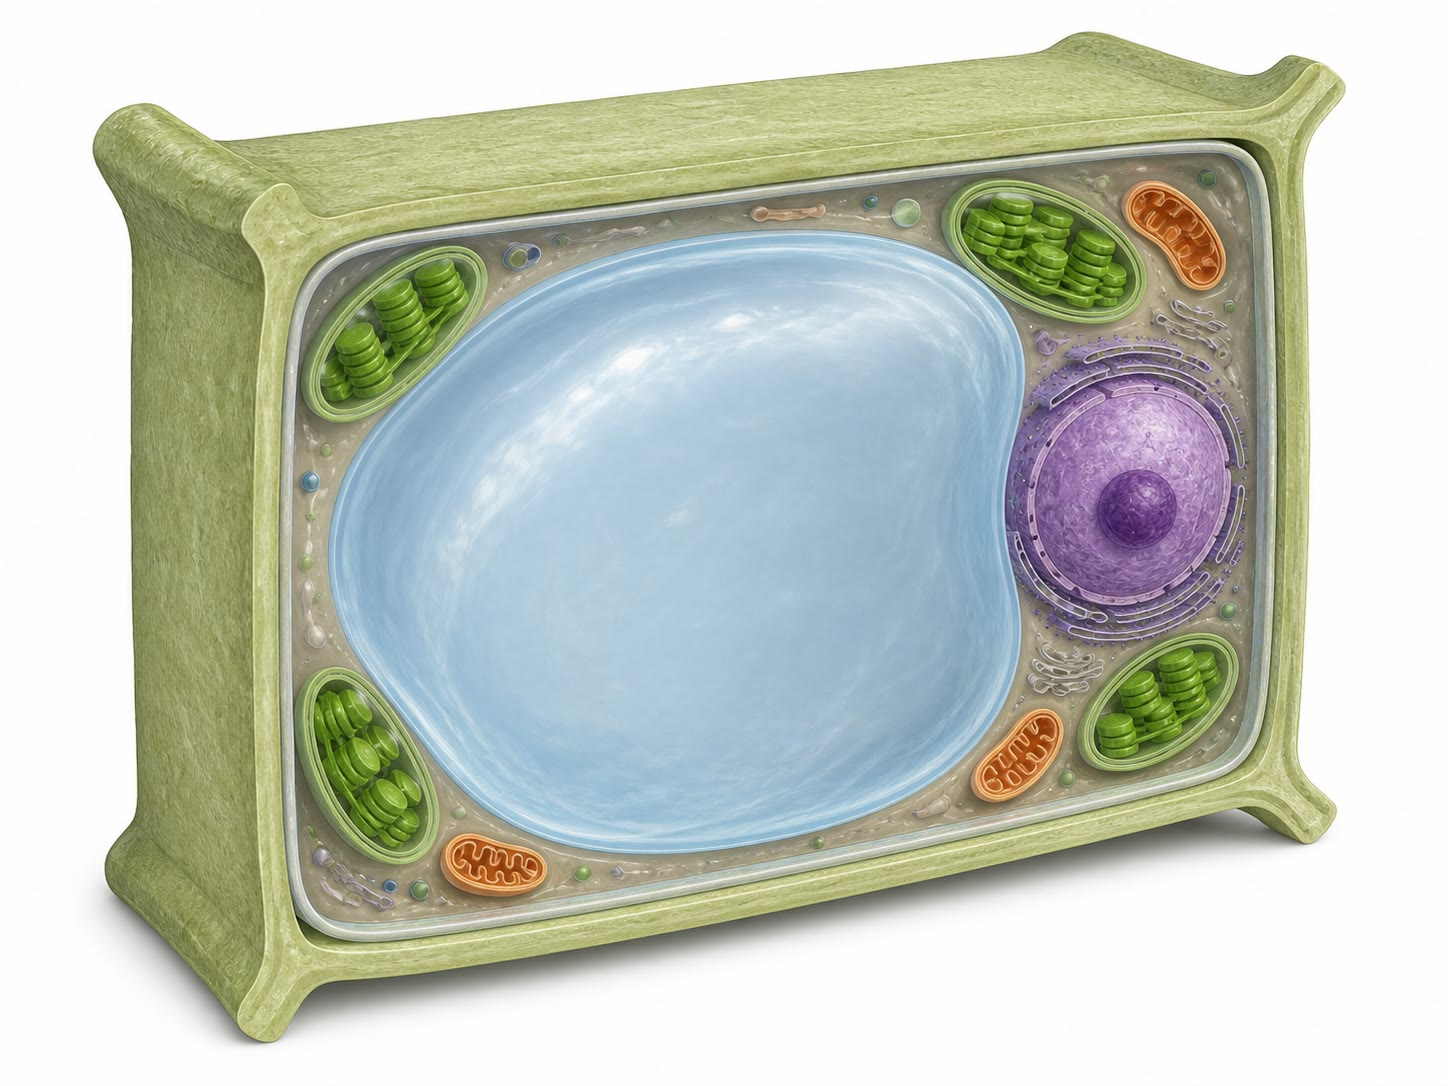
\includegraphics[width=0.52\linewidth]{images/book2/ai/fig-plant-cell-cutaway-v2.jpg}};
  \begin{scope}[x={(img.south east)}, y={(img.north west)},
      every node/.style={font=\small}]
    \draw[omDef, thick] (0.50,0.50) -- (0.50,1.08) node[above] {vakuola pusat};
    \draw[omDef, thick] (0.10,0.50) -- (-0.03,0.56) node[left] {dinding sel};
    \draw[omDef, thick] (0.25,0.73) -- (-0.03,0.84) node[left] {kloroplas};
    \draw[omDef, thick] (0.35,0.17) -- (-0.03,0.12) node[left] {mitokondria};
    \draw[omDef, thick] (0.76,0.47) -- (1.03,0.60) node[right] {inti};
    \draw[omDef, thick] (0.60,0.13) -- (1.03,0.16) node[right] {sitoplasma tipis};
  \end{scope}
\end{tikzpicture}

{\small Sebuah \omterm{def:b1:cell-unit-of-life:cell}{sel} tumbuhan: dindingnya di luar membrannya, \omterm{def:b1:eukaryotic-cell:plantcell}{vakuolanya}
yang memenuhi sebagian besar volumenya, \omterm{def:b1:eukaryotic-cell:plastid}{kloroplas} dan \omterm{def:b1:eukaryotic-cell:mitochondrion}{mitokondrianya} di
dalam lapisan tipis \omterm{def:b1:cell-unit-of-life:cell}{sitoplasma} di antara keduanya.}
\end{omfigure}

\begin{proposition}[Sel tumbuhan dan sel hewan dibandingkan]\label{prop:b1:eukaryotic-cell:compare}
Keduanya memiliki \omterm{def:b1:cell-unit-of-life:prokeuk}{inti}, RE, Golgi, \omterm{def:b1:eukaryotic-cell:mitochondrion}{mitokondria}, \omterm{def:b1:eukaryotic-cell:peroxisome}{peroksisom}, ribosom dan
\omterm{def:b1:eukaryotic-cell:cytoskeleton}{rangka sel}. \omterm{def:b1:cell-unit-of-life:cell}{Sel} tumbuhan memiliki dinding selulosa, sebuah \omterm{def:b1:eukaryotic-cell:plantcell}{vakuola}
besar, \omterm{def:b1:eukaryotic-cell:plastid}{plastida} dan plasmodesmata, serta tidak memiliki sentriol maupun
\omterm{def:b1:eukaryotic-cell:endomembrane}{lisosom} (\omterm{def:b1:eukaryotic-cell:plantcell}{vakuolanya} yang mencerna); ia tidak merayap maupun menelan, dan
membelah dengan membangun sebuah dinding baru di tengahnya. \omterm{def:b1:cell-unit-of-life:cell}{Sel} hewan
tidak memiliki dinding (sehingga ia dapat berubah bentuk, merayap dan
memfagosit), memiliki \omterm{def:b1:eukaryotic-cell:endomembrane}{lisosom}, sebuah \omterm{def:b1:eukaryotic-cell:cytoskeleton}{sentrosom} dengan sentriol, dan
berhubungan lewat sambungan alih-alih lewat plasmodesmata; ia membelah
dengan menjepit dirinya menjadi dua.
\end{proposition}

\begin{example}[Turgor]\label{ex:b1:eukaryotic-cell:turgor}
Sebuah \omterm{def:b1:cell-unit-of-life:cell}{sel} \omterm{def:b1:flowering-plant-organization:organs}{daun} yang \omterm{def:b1:eukaryotic-cell:plantcell}{vakuolanya} memegang \qty{0.3}{mol/L} zat terlarut
menarik air masuk sampai dindingnya mendorong balik dengan tekanan
sekitar \qty{0.7}{MPa}, yakni tujuh atmosfer; \omterm{def:b1:cell-unit-of-life:cell}{sel} itu lalu menegang dan
\omterm{def:b1:flowering-plant-organization:organs}{daunnya} kukuh. Kekurangan air, \omterm{def:b1:eukaryotic-cell:plantcell}{vakuolanya} kehilangan volume, tekanannya
turun ke nol, dan \omterm{def:b1:flowering-plant-organization:organs}{daunnya} layu --- dindingnya tak berubah, tekanannya
lenyap (\cref{ch:b1:membranes-transport}). Sebuah \omterm{def:b1:cell-unit-of-life:cell}{sel} hewan dalam
larutan yang sama, karena tidak berdinding, akan begitu saja pecah.
\end{example}

\section{Latihan}

\begin{exercise}[$\star$]\label{exo:b1:eukaryotic-cell:1}
Sebutkan \omterm{def:b1:eukaryotic-cell:organelle}{organel} berbatas membran sebuah \omterm{def:b1:cell-unit-of-life:cell}{sel} hewan dan fungsi utama
masing-masing dalam beberapa kata.
\end{exercise}

\begin{exercise}[$\star$]\label{exo:b1:eukaryotic-cell:2}
Runutlah lintasan sebuah enzim pencernaan dari sintesisnya sampai ke
salurannya, dengan menamai tiap ruang dan cara protein itu berpindah di
antaranya.
\end{exercise}

\begin{exercise}[$\star$]\label{exo:b1:eukaryotic-cell:3}
Dari gambar neraca membran, berapa fraksi membran \omterm{def:b1:cell-unit-of-life:cell}{sel} itu yang bersifat
\omterm{def:b1:eukaryotic-cell:mitochondrion}{mitokondria} (membran luar ditambah membran dalam)? Mengapa membran
dalamnya jauh lebih luas daripada membran luarnya?
\end{exercise}

\begin{exercise}[$\star$]\label{exo:b1:eukaryotic-cell:4}
Sebutkan tiga struktur yang dimiliki \omterm{def:b1:cell-unit-of-life:cell}{sel} tumbuhan tetapi tidak dimiliki
\omterm{def:b1:cell-unit-of-life:cell}{sel} hewan, dan dua yang dimiliki \omterm{def:b1:cell-unit-of-life:cell}{sel} hewan tetapi tidak dimiliki \omterm{def:b1:cell-unit-of-life:cell}{sel}
tumbuhan.
\end{exercise}

\begin{exercise}[$\star\star$]\label{exo:b1:eukaryotic-cell:5}
Dari gambar denyut dan pengejaran, pada waktu berapa tandanya memuncak
di RE, di Golgi, dan di butirannya? Perkirakan waktu singgah dari RE ke
butiran dan waktu sebelum separuh tandanya disekresikan.
\end{exercise}

\begin{exercise}[$\star\star$]\label{exo:b1:eukaryotic-cell:6}
Sebuah \omterm{def:b1:cell-unit-of-life:cell}{sel} diperlakukan dengan obat yang membongkar \omterm{def:b1:eukaryotic-cell:cytoskeleton}{mikrotubulnya}.
Ramalkan pengaruhnya pada letak Golgi, pada lalu lintas vesikel, pada
pembelahan \omterm{def:b1:cell-unit-of-life:cell}{sel} dan pada kibasan silianya.
\end{exercise}

\begin{exercise}[$\star\star$]\label{exo:b1:eukaryotic-cell:7}
Sebutkan empat bukti bagi asal usul bakteri \omterm{def:b1:eukaryotic-cell:mitochondrion}{mitokondria}, dan jelaskan
mengapa sebuah \omterm{def:b1:eukaryotic-cell:mitochondrion}{mitokondria} tetap saja tidak sanggup hidup di luar
sebuah \omterm{def:b1:cell-unit-of-life:cell}{sel}.
\end{exercise}

\begin{exercise}[$\star\star$]\label{exo:b1:eukaryotic-cell:8}
Lumen RE ``secara topologis berada di luar \omterm{def:b1:cell-unit-of-life:cell}{sel}''. Jelaskan ungkapan itu
dengan mengikuti sebuah protein membran yang rantai gulanya menghadap
lumen dari RE sampai ke membran plasma: menghadap sisi mana gula itu
pada akhirnya?
\end{exercise}

\begin{exercise}[$\star\star$]\label{exo:b1:eukaryotic-cell:9}
Sebuah \omterm{def:b1:cell-unit-of-life:cell}{sel} yang menyekresi melepas \qty{2000}{} butiran bergaris tengah
\qty{1}{\micro m} tiap hari lewat permukaan apikal seluas
\qty{40}{\micro m^2}. Hitunglah membran yang ditambahkan tiap hari dan
berapa kali permukaan apikalnya harus didaur ulang. Apa siratannya?
\end{exercise}

\begin{exercise}[$\star\star\star$]\label{exo:b1:eukaryotic-cell:10}
Dalam sebuah tabung uji yang memuat ribosom, mRNA sebuah protein
sekresi dan asam amino, hasilnya adalah rantai sepanjang \qty{320}{}
residu; dengan vesikel RE ditambahkan, muncul rantai sepanjang
\qty{300}{} residu di dalam vesikelnya yang tidak dicerna protease yang
ditambahkan sesudahnya. Tafsirkan tiap pengamatan, dan sebutkan apa
yang akan dilakukan sebuah mutan yang kehilangan dua puluh residu
pertamanya.
\end{exercise}

\begin{exercise}[$\star\star\star$]\label{exo:b1:eukaryotic-cell:11}
\omterm{def:b1:cell-unit-of-life:cell}{Sel} seorang pasien kehilangan sebuah enzim \omterm{def:b1:eukaryotic-cell:endomembrane}{lisosom} yang menguraikan
sejenis lipid; lipid itu menumpuk dalam \omterm{def:b1:eukaryotic-cell:endomembrane}{lisosom} yang membengkak dan
\omterm{def:b1:cell-unit-of-life:cell}{selnya} mati. Jelaskan biologi \omterm{def:b1:cell-unit-of-life:cell}{selnya}, sebutkan mengapa penyakitnya
paling parah pada \omterm{def:b1:cell-unit-of-life:cell}{sel} yang memperbarui membrannya paling cepat, dan
ajukan bagaimana sebuah enzim yang disuntikkan ke dalam darah dapat
mencapai \omterm{def:b1:eukaryotic-cell:endomembrane}{lisosomnya}.
\end{exercise}

\begin{exercise}[$\star\star\star$]\label{exo:b1:eukaryotic-cell:12}
``\omterm{def:b1:cell-unit-of-life:prokeuk}{Sel eukariot} adalah sebuah federasi bekas bakteri yang disatukan
sebuah sistem membran.'' Bahaslah dalam satu paragraf, dengan menimbang
apa yang dijelaskan teori endosimbiosis terhadap apa yang tidak
dijelaskannya (\omterm{def:b1:cell-unit-of-life:prokeuk}{inti}, RE, \omterm{def:b1:eukaryotic-cell:cytoskeleton}{rangka sel}).
\end{exercise}

\section{Soal: Sel Asinus Pankreas}

\begin{problem}[{Soal akhir pekan --- sebuah sel yang menyekresi
protein sebanyak massanya sendiri tiap hari: jam Palade, membran yang
harus didaur ulangnya, isyarat yang mengarahkan proteinnya, berakhir
pada waktu singgah sebuah enzim pencernaan}]
\label{pb:b1:eukaryotic-cell:1}
Sebuah \omterm{def:b1:cell-unit-of-life:cell}{sel} asinus pankreas adalah kubus bersisi \qty{12}{\micro m},
dengan sisi apikalnya (\qty{144}{\micro m^2}, pada salurannya) dan sisi
basalnya pada darah. Sebuah pankreas manusia \qty{80}{g} memuat sekitar
$\num{8e10}$ \omterm{def:b1:cell-unit-of-life:cell}{sel} semacam itu dan menyekresi \qty{10}{g} protein enzim
tiap hari. Sebuah butiran sekresi adalah bola bergaris tengah
\qty{1}{\micro m} yang memegang protein pada \qty{200}{mg/mL}. Ribosom
menambahkan \qty{5}{} asam amino tiap sekon; sebuah enzim yang lazim
memiliki \qty{250}{} residu bermassa rata-rata
\qty{110}{g/mol}.

\medskip
\noindent\textbf{Bagian I --- Jam Palade.}
Gambar denyut dan pengejaran pada bab ini memberikan letak tandanya
terhadap waktu.
\begin{enumerate}
  \item Mengapa denyutnya harus singkat dan pengejarannya harus memuat
        asam amino tak bertanda yang berlebih?
  \item Bacalah waktu ketika tandanya memuncak di RE, di Golgi dan di
        butirannya.
  \item Perkirakan waktu singgah dari RE ke Golgi dan dari Golgi ke
        butiran.
  \item Di mana tandanya pada \qty{60}{min}, dan mengapa sebagian di
        antaranya sudah meninggalkan \omterm{def:b1:cell-unit-of-life:cell}{sel} sementara sebagian besarnya
        masih berada dalam butiran?
  \item Percobaan kedua dilakukan pada \qty{15}{\celsius}: tandanya
        tinggal di RE lebih dari sejam. Tafsirkan.
\end{enumerate}

\medskip
\noindent\textbf{Bagian II --- Massa proteinnya.}
\begin{enumerate}[resume]
  \item Hitunglah protein yang disekresikan tiap \omterm{def:b1:cell-unit-of-life:cell}{sel} tiap hari, dalam
        pikogram.
  \item Hitunglah volume satu butiran dan massa protein yang
        dipegangnya.
  \item Hitunglah banyaknya butiran yang dilepas tiap \omterm{def:b1:cell-unit-of-life:cell}{sel} tiap hari,
        dan tiap menit.
  \item Hitunglah volume \omterm{def:b1:cell-unit-of-life:cell}{sel} itu dan, dengan massa jenis
        \qty{1.05}{g/cm^3}, massanya. Berapa fraksi massanya sendiri
        yang disekresikannya tiap hari?
  \item Hitunglah banyaknya molekul enzim dalam satu butiran (bilangan
        Avogadro $\num{6.0e23}$).
  \item Hitunglah waktu yang dibutuhkan sebuah ribosom untuk membuat
        satu molekul enzim.
  \item Berapa banyak ribosom yang harus bekerja terus-menerus untuk
        membuat keluaran hariannya? Bandingkan dengan $\num{4e6}$
        ribosom yang dimuat \omterm{def:b1:cell-unit-of-life:cell}{sel} semacam itu.
\end{enumerate}

\medskip
\noindent\textbf{Bagian III --- Membran.}
\begin{enumerate}[resume]
  \item Hitunglah luas membran satu butiran.
  \item Hitunglah membran yang diantarkan ke sisi apikalnya tiap hari
        lewat eksositosis butiran pada pertanyaan 8.
  \item Berapa kali sehari luas sisi apikalnya ditambahkan? Apa yang
        harus dilakukan \omterm{def:b1:cell-unit-of-life:cell}{sel} itu dengannya, dan lewat proses apa?
  \item Membran butirannya datang dari Golgi, yang menerimanya dari RE.
        Bila RE \omterm{def:b1:cell-unit-of-life:cell}{sel} itu memiliki \qty{20000}{\micro m^2} membran, itu
        setara membran butiran berapa hari? Apa yang dikatakan hal ini
        tentang pendauran ulang di dalam \omterm{def:b1:eukaryotic-cell:endomembrane}{sistem endomembrannya}?
  \item Sisi apikalnya membawa \qty{2000}{} mikrovilus bergaris tengah
        \qty{0.1}{\micro m} dan sepanjang \qty{1}{\micro m}. Berapa kali
        lipat mikrovilus itu memperluas sisi \qty{144}{\micro m^2} tadi?
\end{enumerate}

\medskip
\noindent\textbf{Bagian IV --- Alamat pada proteinnya.}
\begin{enumerate}[resume]
  \item mRNA sebuah enzim yang ditranslasikan dalam tabung uji tanpa
        membran memberikan rantai yang \qty{20}{} residu lebih panjang
        daripada enzim yang ditemukan dalam butirannya. Di mana residu
        tambahan itu dan apakah itu?
  \item Dengan vesikel RE hadir, hasilnya berpanjang tepat, berada di
        dalam vesikelnya, dan terlindung dari sebuah protease.
        Tafsirkan.
  \item Percobaan yang sama dengan mRNA sebuah enzim \omterm{def:b1:eukaryotic-cell:organelle}{sitosol}
        memberikan hasil di luar vesikelnya dan tak terlindung.
        Simpulkan.
  \item Sebuah mutasi menghapus kedua puluh residu itu. Ramalkan di
        mana enzim itu berakhir dan apa yang terjadi pada \omterm{def:b1:cell-unit-of-life:cell}{selnya}.
  \item Sebuah enzim lain ditemukan dalam \omterm{def:b1:eukaryotic-cell:endomembrane}{lisosom} alih-alih dalam
        butirannya. Ia membawa jenis \omterm{prop:b1:eukaryotic-cell:secretory}{urutan isyarat} yang sama. Di
        sebelah mana sepanjang lintasannya keputusan kedua itu harus
        diambil, dan lewat mekanisme apa, secara garis besar?
  \item Sebuah \omterm{def:b1:cell-unit-of-life:cell}{sel} diperlakukan dengan obat yang menghambat sintesis
        ATP. Ramalkan di mana tanda sebuah denyut dan pengejaran
        menumpuk dan mengapa (dua alasan).
  \item Gabungkan pertanyaan 3 dan 8: pada keadaan tunak, berapa banyak
        butiran yang ``sedang dalam perjalanan'' antara RE dan butiran
        pada tiap saat?
  \item Ringkaslah hasilnya: waktu singgah dari sintesis sampai
        butiran, waktu sampai sekresi, butiran yang dilepas tiap menit,
        dan fraksi massanya sendiri yang disekresikan \omterm{def:b1:cell-unit-of-life:cell}{sel} itu tiap hari.
\end{enumerate}
\end{problem}
